\documentclass[letterpaper,12pt]{article}

%\usepackage{amsmath}
%\usepackage[dvips]{graphicx}
\usepackage{hyperref}
%    \hypersetup{colorlinks=true,urlcolor=blue,linkcolor=red}
\RequirePackage{GE05}

\newcommand{\GDP}{\mbox{\em GDP\/}}
\newcommand{\NDP}{\mbox{\em NDP\/}}
\newcommand{\GNP}{\mbox{\em GNP\/}}
\newcommand{\NX}{\mbox{\em NX\/}}
\newcommand{\NY}{\mbox{\em NY\/}}
\newcommand{\CA}{\mbox{\em CA\/}}
\newcommand{\NFA}{\mbox{\em NFA\/}}
\newcommand{\Def}{\mbox{\em Def\/}}
\newcommand{\CPI}{\mbox{\em CPI\/}}
\newcommand{\IP}{\mbox{\em IP\/}}


\def\ClassName{The Global Economy}
\def\Category{Class Notes}
\def\HeadName{Business Cycle Indicators}

\begin{document}
\thispagestyle{empty}%
\Head

\centerline{\large \bf \HeadName}%
\centerline{Revised: \today}

\bigskip
Probably the leading use of macroeconomic data (and macroeconomists) is forecasting:  predicting
future movements in economic variables so that businesses can decide whether to build new plants
or hire new workers, investors can decide how to allocate their assets, and households can decide
how much to spend. The good news is that forecasting is possible;  
we're not simply throwing darts at a board.  
The bad news is that it's not easy.


This set of notes is devoted to short-term (``business cycle'')
indicators:  variables that indicate future movements in the
economy.  In principle we could be interested in many features of
the economy:  output, inflation, exchange rates, and so on. We'll
focus on output and interest rates, using other variables as they
relate to those two. The emphasis is on the US, but similar ideas
and methods apply to other countries.


\subsubsection*{Where are we headed?}

The classic forecasting problem goes something like this:  What do we expect the value of [some
economic variable] to be $k$ periods in the future?  Here $k$ is any period of time you like, but
we're usually interested in the next year or two.

\begin{figure}
    \centering
    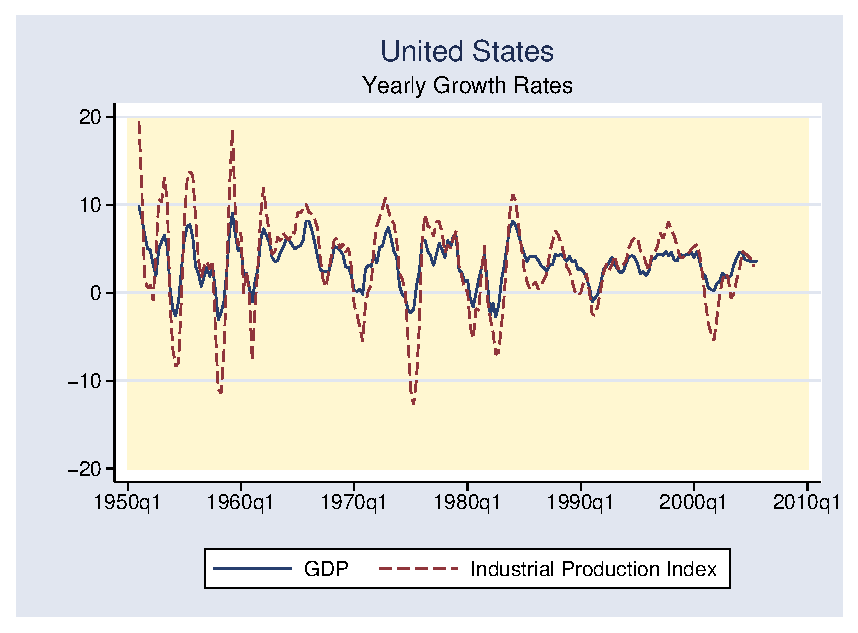
\includegraphics[scale=0.8]{us_gdp_indprod.eps}
    \caption{GDP and Industrial Production.}
    \label{fig:ip_gdp}%
\end{figure}

If we're forecasting GDP, there's an extra difficulty: we don't
know the present or the recent past, much less the future. We've
seen, for example, that fourth-quarter GDP is first reported near
the end of the following January, and even that number is a
preliminary estimate. From the perspective of mid-January, then,
we need to ``forecast'' the previous quarter.

We're going to shortcut this difficulty (somewhat) by using the
monthly Industrial Production (IP) index as a substitute for real
GDP, but the issue is a general one:  the time lag in getting data
is both an issue in its own right and a  constraint on forecasting
the future. IP measures output in manufacturing, mining, and
utilities. More important, its fluctuations are strongly
correlated with those in GDP.  You can see that in
Figure~\ref{fig:ip_gdp}, which compares year-on-year growth rates
in GDP and IP (aggregated to a quarterly frequency). You will
notice that IP is more volatile than GDP but otherwise follows its
ups and downs reasonably well.  You may also notice some
differences between them in the recent past, which have been
traced to the rising importance of services in the US economy.  In
the US, IP is reported by the Federal Reserve in the middle of the
following month.  Data for December, for example, are available in
mid-January.  Using IP therefore gives us a shorter information
lag than GDP.  In addition, the monthly frequency gives us a finer
time interval for near-term forecasting.  For both reasons, we
will focus our discussion of forecasting on IP rather than GDP,
although the same principles apply to both, as well as to other
macroeconomic and financial variables.


Many countries report similar measures of industrial production. A good source for developed
economies is the OECD's
\href{http://www.oecd.org/document/54/0,2340,en_2649_37461_15569334_1_1_1_37461,00.html}{\it Main
Economic Indicators\/}.


\subsubsection*{Good indicators}

%
\begin{table}
\begin{center}
\begin{tabular}{lc}
\hline\hline Indicator   & Weight  \\
\hline\hline
Average weekly hours, manufacturing  &  0.1946  \\
Average weekly initial claims for unemployment insurance & 0.0268 \\
Manufacturers' new orders, consumer goods and materials & 0.0504
\\
Vendor performance, slower deliveries diffusion index &  0.0296
\\
Manufacturers' new orders, non-defense capital goods &  0.0139
\\
Building permits, new private housing units &  0.0205 \\
Stock prices, 500 common stocks &  0.0309 \\
Money supply, M2 & 0.2775 \\
Interest rate spread, 10-year Treasury bonds less federal funds &
0.3364 \\
Index of consumer expectations & 0.0193 \\
\hline\hline
\end{tabular}
\end{center}
\caption{Components of the Conference Board's US Leading
Indicators} \label{tab:lei}
\end{table}
%

Good forecasts require good inputs.  One way to forecast a
variable is to use its own past.  Future growth rates in IP, for
example, might be related to current and past growth rates. We can
usually do better than that by adding other ``indicators'' to our
analysis.  We've seen, for example, that fluctuations in average
hours in manufacturing, the S\&P 500 index, and yield spreads lead
fluctuations in output, so these variables are good candidates.
More generally, a good indicator should have one or more of these
properties:
%
\begin{itemize}

\item Correlation.  A good indicator is correlated with the
variable we are forecasting.

\item Lead. A good indicator leads the variable we are
forecasting.

\item Timeliness.  A good indicator is available quickly.

\item Stability.  A good indicator does not undergo major
revisions subsequent to its initial release.

\end{itemize}
On the whole, economic indicators (average hours, retail sales)
tend to be strong on correlation, weak on timeliness (see the
discussion of GDP above) and stability (many economic series are
revised frequently). The best ones lead the business cycle.  In
contrast, financial indicators (equity prices, interest rates) are
weaker on correlation but stronger on the other three properties:
they're typically available immediately, often lead the cycle, and
are not revised.


Indexes of leading indicators combine multiple series with the
hope of getting the best from each.  The Conference Board's
quasi-official index of leading indicators is a weighted average
of ten individual indicators;  see Table~\ref{tab:lei}. It
includes both financial indicators (stock prices, the term spread)
and economic indicators (average weekly hours in manufacturing,
initial claims for unemployment insurance).  The weight tells us
the importance of each series: the growth rate of the index is the
weighted average of the growth rates of the individual series,
after each series has been divided by its standard deviation.  (If
this seems confusing, don't worry about it --- it's a fine point.)


The individual series listed in Table~\ref{tab:lei} reflect the
properties of good indicators.  Average weekly hours, as we've
seen, is closely correlated with, and leads, the business cycle.
It comes from a survey conducted by the Bureau of Labor Statistics
and is available less than a week following the month to which it
refers.  Revisions occur, but they're usually modest. Average
weekly new claims for unemployment insurance is available weekly
but is similar in other respects.  The term spread is available
immediately and leads the cycle, but is less highly correlated
with output than (say) average hours.  M2 is a measure of the
``money supply,'' which consists of currency, checking accounts,
savings accounts, and small-denomination time deposits. The
Federal Reserve releases weekly report of monthly data, with the
first estimates available 1-2 weeks after the relevant month.


Similar series are available for other countries from many
sources. Among the most popular:  the %
\href{http://www.conference-board.org/economics/bci/}{Conference
Board} constructs and reports business cycle indicators for nine
countries, available by subscription.  The %
\href{http://www.oecd.org/department/0,2688,en_2649_34349_1_1_1_1_1,00.html}{OECD}
constructs its own indexes for 20+ developed countries. A variety
of private services construct indicators for real output,
inflation, and other variables of interest.  The most interesting
is %
\href{http://www.businesscycle.com/}{ECRI}, whose indicators have
done extremely well over the last decade.


\subsubsection*{Regression-based forecasting}

Now that we have some indicators, how do we use them?  Let us say,
to be concrete, that we are forecasting  the multi-period growth
rate of industrial production. We compute the (annualized) growth
rate this way:
\[
    \gamma_{t,t+k} \;=\; \log (\IP_{t+k}/\IP_t) \times (12/k) .
\]
We refer to $k$ (here measured in months) as the {\it forecast
horizon\/}.  The adjustment factor ``$12/k$'' converts the growth
rate to annual units.

The standard way to construct a forecast is to base it on a
regression.  To forecast IP growth, we would estimate a regression
of the form
\[
        \gamma_{t,t+k}  \;=\;  a + b x_t + \mbox{residual},
\]
where $x_t$ is the value of an indicator at date $t$ (``now,''
when the forecast is made).  We use a sample of data to estimate
the parameters $a$ and $b$, then forecast the future by using the
current value of $k$ to estimate future growth:
\[
        \widehat{\gamma}_{t,t+k}  \;=\;  \widehat{a} + \widehat{b} \; x_t .
\]
(The ``hats'' remind us we are using estimates.)  Variants of this
approach add multiple indicators and/or past values of $\IP$ and
indicators to the regression.


%
\begin{table}
\begin{center}
\setlength{\tabcolsep}{0.20in}
\begin{tabular}{ccccc}
\hline\hline
Horizon &  \multicolumn{2}{c}{Interest Rate Spread} & \multicolumn{2}{c}{Leading Indicators}\\
\cline{2-3} \cline{4-5}
(months)    &          Std Error                  &   $ R^2 $ &          Std Error        &   $ R^2 $\\
\hline\hline
         1        &          0.104               &    0.050  &          0.098                     &   0.001  \\
         2        &          0.085               &    0.079  &          0.081                     &   0.001 \\
         3        &          0.076               &    0.107  &           0.073                   &    0.002\\
         4         &          0.069               &    0.134  &           0.067                   &  0.002\\
         5        &          0.064               &    0.156  &           0.062                   &  0.003\\
         6        &          0.059               &    0.177  &          0.058                    &  0.004 \\
         7         &          0.055               &    0.196  &           0.054                   &  0.005\\
         8        &          0.052               &    0.213  &           0.052                   &   0.007\\
         9        &          0.049               &    0.226  &           0.050                   & 0.010\\
         10         &         0.047               &    0.237  &            0.048                  & 0.013\\
         11        &         0.045               &    0.247  &            0.047                  & 0.016\\
         12        &         0.043               &    0.255  &            0.045                  & 0.019\\
         13         &         0.041               &    0.260  &            0.044                  & 0.012\\
         14        &         0.040               &    0.264  &            0.042                  & 0.024\\
         15        &         0.038               &    0.271  &            0.041                   &  0.028\\
         16         &         0.037               &    0.280  &            0.040                  &  0.031\\
         17        &         0.035               &    0.289  &            0.039                  & 0.035\\
         18        &         0.034               &    0.296  &            0.038                  & 0.040\\
         19         &         0.033               &    0.300  &            0.037                 & 0.045\\
         20        &         0.032               &    0.299  &             0.036                 & 0.050\\
         21        &         0.031               &    0.298  &             0.035                  & 0.056\\
         22         &         0.030               &    0.292  &            0.034                  & 0.062\\
         23        &         0.030               &    0.283  &             0.033                 & 0.068\\
         24        &         0.029               &    0.272  &            0.032                  & 0.075\\
         25         &         0.029               &    0.262  &            0.032                  & 0.083\\
         26        &         0.028               &    0.253  &             0.031                 & 0.090\\
         27        &         0.028               &    0.243  &           0.030                   & 0.098\\
         28        &         0.027               &    0.235  &           0.029                   & 0.105\\
         29        &         0.027               &    0.227  &            0.028                  & 0.112\\
         30         &         0.026               &    0.220  &            0.028                  & 0.118\\
         31        &         0.026               &    0.211  &            0.027                  & 0.124\\
         32        &         0.025               &    0.203  &            0.026                  & 0.129\\
         33         &         0.024               &    0.195  &            0.026                  & 0.135\\
         34        &         0.024               &    0.190  &            0.025                  & 0.140\\
         35        &         0.024               &    0.185  &            0.025                 & 0.144\\
         36        &         0.023               &    0.181  &            0.024                  & 0.149\\
\hline\hline
\end{tabular}
\end{center}
\caption{Forecasting Growth in Industrial Production.  Entries
summarize forecasting regressions for the growth rate of
industrial production. One set of regressions is based on the term
spread, the other on the index of leading indicators.  Both are
reported for forecasting horizons of 1 to 36 months.  The sample
period is 1950-2004.}

\label{tab:forecast}
\end{table}


We report some of the properties of two such ``forecasting
regressions'' in Table~\ref{tab:forecast}. The first uses the term
spread as the indicator $x$, the second uses the index of leading
indicators. In each case, we estimate the regression for forecast
horizons of 1 to 36 months. The regressions suggest, first, that
the indicators have some forecasting power.  For time horizons
between 12 and 24 months, the $R^2$s imply that we are explaining
25-30\% of the variation in the growth of industrial production.
We might expect to do worse out of sample, but it's a sign that
the business cycle is at least partly predictable.  The
regressions also suggest that forecasting is imperfect:  the
standard error of the 24-month forecast is about 3\%, so the
95-percent confidence interval is enormous. For example, suppose
we forecast 5\% growth.  Then a plus-or-minus-two-standard
deviation confidence interval ranges from --1\% to +11\%! In
short, we can forecast future growth in IP, but a lot of the
future remains unpredictable --- at least with these indicators.


Some of the best forecasts aggregate information from multiple
sources.  Indexes of leading indicators do this one way:  they
combine various indicators to produce an index, which is then used
to forecast the future.  Another approach is to aggregate the
forecasts themselves.  The so-called ``Blue Chip" forecast is an
average of forecasts generated by experts, and it performs better,
on average, than any single forecaster.  Some statistical
forecasters do the same sort of thing on their own:  they generate
multiple forecasts with methods like our forecasting regression,
then average them to generate a final aggregate forecast. Again,
the aggregate tends to do better than the individual forecasts.

A related idea is to rely on markets, which aggregate information
from a variety of sources.  Presidential futures markets, for
example, have predicted the popular vote in the last four
elections more accurately than any of the major polls.  In the
economic arena, the CME has futures on the CPI, and there has been
talk of future markets for a variety of short-term economic
indicators. (The economic and financial contracts on
\href{http://www.tradesports.com/jsp/intrade/contractSearch/}{Tradesports.com}
show how this might work.)  The logic is compelling: futures
markets, by aggregating information from a wide range of sources,
are often good indicators of the future.  They're not perfect ---
the future will always be somewhat unpredictable
--- but they're often close to the best we can do.



\subsubsection*{The yield curve}


We turn next to the yield curve, which we use to infer ``the
market's'' forecast of future interest rates.  In this case we're
using market prices to aggregate the various kinds of information
available to market participants. Roughly speaking, the slope of
the yield curve tells us what the market expects of future
short-term interest rates. But before we explain how this works,
we need to review yields and forward rates.

Yields and forward rates are subspecies of interest rates. {\it
Yields\/} are simply a way of reporting bond prices. If you go
into the bond business you'll find there are lots of details to
worry about (accrued interest, day count conventions, etc), but
we'll keep it simple and look at yields on bonds with no coupons
--- zero-coupon bonds or ``zeros.''  A one-year zero is a claim to (say) \$100 in
one year.  A two-year zero is a claim to \$100 in two years.  An
$m$-year zero is a claim to \$100 in $m$ years, and so on.  If the
price of an $m$-year bond is $p_m$, its yield $y_m$ is defined by
the present value formula:
\begin{equation}
        p_m  \;=\; 100/(1+y_m)^m.
        \label{eq:pv}
\end{equation}
This formula is based on annual compounding, which is the most
convenient convention for our purposes; more on this shortly. Note
that if we know prices, we can find yields, and vice versa. The
{\it yield curve\/} for zero-coupon bonds is a graph of yield
$y_m$ versus maturity $m$.


The yield curves you see in the newspaper are usually based on
yields of coupon bonds, and in the case of US treasuries they use
semi-annual compounding. They capture similar information, but
they're a little harder to make sense of.  Why?  Because the yield
depends not only on maturity, it also depends on the coupon. Since
the coupons vary over time and across maturities, it's never
exactly clear what we're talking about.  For that reason, most
formal fixed income analysis starts with prices and yields of
zeros.


{\em Example.} Suppose prices of zero-coupon bonds are
%
\begin{center}
\begin{tabular}{cc}
                    Maturity        &     Price         \\
                             1              &      94.24        \\
                             2              &      87.70        \\
                             3              &      81.22        \\
                             4              &      75.16        \\
                             5              &      69.66
\end{tabular}
\end{center}
%
What are the yields?

Answer.  The yields are 6.11, 6.78, 7.18, 7.40, and 7.50,
respectively, expressed as annual percentages.  The third one
solves the equation $ 81.22 = 100/(1+y_3)^3 $, namely $ 1 + y_3 =
(100/81.22)^{1/3} $.  The others are similar.



Yields are interest rates that apply over a number of periods. For
example, the $m$-year yield at date $t$ applies over the period of
time between $t$ (now) to $t+m$ ($m$ years from now).  One way to
think about the return on the bond is that the invests $p$ and
gets a rate of return equal to the yield $y$ for every period
until maturity.  In the two-period case, this leads to
\[
    100 \;=\; p_2 \times (1+y_2) (1+y_2) ,
\]
a variant of our present value formula, equation (\ref{eq:pv}).
Another way to think about the return is that the rates vary
across periods. In the two-period case, the bond might have
different rates of return in the first and second periods. But
what are these returns?  We know the return on a one-period bond
is $y_1$, so the first-period return should be $y_1$.  What about
the second period?  We need an interest rate that applies to the
second period alone but that remains consistent with the price of
the bond. That is, a rate $f_1$ that satisfies
\[
    100 \;=\; p_2 \times (1+y_1) (1+f_1) .
\]
Putting these two equations together tells us
\[
    (1+y_2)^2 \;=\; (1+y_1) (1+f_1)
\]
or
\[
    1+f_1 \;=\; p_1/p_2 .
\]
We refer to $f_1$ as the one-period-ahead {\it forward rate\/},
since it applies at date $t$ to the time period between $t+1$ and
$t+2$. It's the rate of return on a {\it forward contract\/} in
which we agree at $t$ to invest a fixed amount at $t+1$ for one
period.


The same logic applies to bonds with maturities greater than two.
The bond price can be expressed as
\begin{eqnarray*}
        p_m &=& 100/(1+y_m)^m \\
            &=& 100/ [(1+y_1)(1+f_1) \cdots (1+f_{m-1})] .
\end{eqnarray*}
The two relations together imply
\begin{equation}
    1+f_{m-1} \;=\; p_{m-1}/p_{m} ,
    \label{eq:fdef}
\end{equation}
where $f_m$ is the $m$-period-ahead forward rate.  Draw a circle
around this equation: you'll be using it soon.  What we're doing
here is using bonds of two consecutive maturities to ``pick off''
the forward rate that applies over the last period.


Putting all the pieces together, we have three ways to express the
same information:  bond prices, yields, and forward rates. Given
data on a complete set of maturities, we can compute any one of
the three from any other.


{\it Example (continued).\/} For the bond prices and yields
reported earlier, verify that the forward rates are
%
\begin{center}
\begin{tabular}{cccc}
  Maturity ($m$)  &  Price ($p_m$)  &  Yield ($y_m$)  & Forward Rate ($f_{m-1}$) \\
     1      &  94.24  &   6.11 &   6.11    \\
     2      &  87.70  &   6.78 &   7.45         \\
     3      &  81.22  &   7.18 &   7.98     \\
     4      &  75.16  &   7.40 &   8.06       \\
     5      &  69.66  &   7.50 &   7.90
\end{tabular}
\end{center}
Note that the maturities of forward rates are one less than those
of bond prices and yields.  We do this because they naturally
start at zero, for reasons that may be clearer to you shortly. The
0-period-ahead forward rate is simply the current one-period
yield:   $f_0 = y_1$.

Answer.  We compute forward rates from prices.  For $m=5$, the
calculation implied by equation (\ref{eq:fdef}) is
\[
    1 + 0.0790 \;=\; 75.16/69.66.
\]
The others are similar.


\subsubsection*{Reading the yield curve}

Now that we've done all this work, we can use it to predict future
one-period yields.  Put simply but somewhat imprecisely, we're
going to say that forward rates are the market's expectation of
future one-period yields, plus an adjustment for risk that depends
on maturity but doesn't vary over time.  Once we've done the
adjustment, we can read expected future one-period yields from the
forward rate curve. The idea is referred to as the {\it
expectations hypothesis\/} because it's based on the premise that
forward rates include expectations of future one-period yields ---
{\it short rates\/} in conventional terminology.

To be more precise we need to add a little notation. Since we'll be dealing a lot with the
one-period yield or short rate, let us label it $i$, so that $i_t$ is the yield on a one-period
bond bought at date $t$. We label (one-period) forward rates by $f_{m,t}$, meaning the rate on a
forward contract arranged at date $t$ but applying to the period between dates $t+m$ and $t+m+1$.
The expectations hypothesis states that the forward rate is the market's expectation or forecast
of the future short rate plus a risk premium:
\begin{equation}
    f_{m,t} \;=\; E_t (i_{t+m}) + \mbox{risk premium}_m .
    \label{eq:eh}
\end{equation}
The risk premium is assumed to be constant across time but may
vary by maturity.  The notation $E_t$ is meant to convey the
expectation made at date $t$.  If we know forward rates and risk
premiums, we can compute expected future short rates.


That's what the expectations hypothesis is, but where does it come
from?  Let's think about what an investor would demand of a
forward rate.  An investor with a two-period time horizon has (at
least) two choices.  She could buy and hold a two-period bond at
date $t$, thus getting (according to our second interpretation)
returns of $ i_t $ in the first period and $ f_{1,t} $ in the
second.  Alternatively, she could roll over a one-period bond,
getting (again) $ i_t $ the first period and the short rate $
i_{t+1} $ in the second.  These two possibilities can be pictured
like this:
%
\begin{center}
\unitlength=0.6mm
\begin{picture}(100,50)
  \put(50,45){\makebox(0,0){Rollover Strategy}}
  \put(25,32){\makebox(0,0){$i_t$}}
  \put(75,32){\makebox(0,0){$i_{t+1}$}}
  \put(0,25){\line(100,0){100}}
  \put(0,25){\makebox(0,0){$ | $}}
  \put(50,25){\makebox(0,0){$ | $}}
  \put(100,25){\makebox(0,0){$ | $}}
  \put(25,18){\makebox(0,0){$i_t$}}
  \put(75,18){\makebox(0,0){$f_{1,t}$}}
  \put(50,5){\makebox(0,0){Buy and Hold Strategy}}
\end{picture}
\end{center}
%
If $ i_{t+1} $ were known, then we would expect the market to
drive the forward rate $ f_{1,t} $ and the future short rate $
i_{t+1} $ together:  $ f_{1,t} = i_{t+1} $. If the future short
rate were higher, then no one would buy the long bond.  Its price
would fall and the forward rate would rise.  If it were lower,
everyone would buy the long bond and bid up its price. In an
uncertain world, similar logic might lead us to guess that the
forward rate is the market's forecast of the future short rate,
with some adjustment for risk:
\[
    f_{1,t}   =  E_t ( i_{t+1} ) + \mbox{\em risk premium}   .
\]
Similar reasoning for longer maturities leads us to equation
(\ref{eq:eh}).


The only remaining issue is estimating the risk premiums.  There
are as many ways to do this as there are finance professors, but a
relatively simple method is to use the average difference between
the short rate and the $n$-period forward rate as an estimate of
its risk premium; that is, we use
\begin{equation}
    \mbox{risk premium}_m  \;=\; E (f_{m,t}  -  i_{t} )
\end{equation}
and estimate the expectation on the right with the mean. This
should work as long as forecast errors (the difference between the
future short rate and its expectation) are zero, on average, and
the distribution of the short rate doesn't change over time (the
means of the short rate and future short rate are the same).
Table~\ref{tab:meanrates} summarizes mean forward rates for US
treasuries for the period 1970-2000.  Since the short rate is the
first forward rate, we compute risk premiums by subtracting it
from the other forward rates.

\begin{table}[h]
\centering
\begin{tabular}{ccc}
\hline\hline
        Maturity   &    Mean Forward Rate   &  Risk Premium \\
\hline\hline
            1  &  7.51 &  0.00 \\
            2  &  8.10 &  0.59 \\
            3  &  8.39 &  0.88 \\
            4  &  8.57 &  1.06 \\
            5  &  8.67 &  1.16  \\
\hline\hline
\end{tabular}
\caption{Mean Forward Rates for US Treasuries, 1970-2000.}
\label{tab:meanrates}
\end{table}


{\it Example (continued again).\/} For the forward rates reported
earlier, what are the implied expected future short rates?

Answer.  The calculations are summarized by
%
\begin{center}
%\newlength{\oldtab}
%\setlength{\oldtab}{\tabcolsep} \setlength{\tabcolsep}{0.10in}
\begin{tabular}{cccc}
  Maturity ($m$) & Forward Rate ($f_{m-1}$) & Risk Premium & Future Short Rate ($i_{t+m-1}$) \\
     1      &   6.11       &    0.00      &    6.11 \\
     2      &   7.45       &    0.59      &    6.86  \\
     3      &   7.98       &    0.88      &    7.10  \\
     4      &   8.06       &    1.06      &    7.00  \\
     5      &   7.90       &    1.16      &    6.74
\end{tabular}
\end{center}
%\setlength{\tabcolsep}{\oldtab}
%

In short, we can read expected future short-term interest rates
from the forward rate curve, which we compute from the yield curve
for zeros.  If you find this interesting, there's a lot more on
related topics in the Debt Instruments course.


\subsubsection*{Executive summary}

\begin{enumerate}
\item Fluctuations in economic activity can be (partially)
predicted by a number of indicators:  the term spread, new
unemployment claims, stock prices, and so on.

\item Indexes of leading indicators typically combine a number of
such indicators into a single index.

\item We can generate forecasts with regressions, which relate
future values of a variable of interest to the current value of
one or more indicators.

\item The yield curve can be used to infer market expectations of
future short-term interest rates.

\end{enumerate}


\subsubsection*{Review questions}

\begin{enumerate}

\item Building permits on new private housing is one of the
components of the leading indicators.  In what ways do you think
it would be a good indicator?  A bad one?  Further information is
available at the US Census Bureau's
\href{http://www.census.gov/const/www/newresconstindex.html}{web
site}.

Answer.  Good:  connected to housing, which as a durable good
should be cyclically sensitive and volatile; available quickly; it
leads the cycle (which you wouldn't know). Bad: based on a sample,
which leads to short-term noise; revised periodically.

\item In 2002, a government agency recommended that we establish a
futures market in terrorist attacks, on the grounds that it would
give us a useful public indicator of their likelihood.  The idea
was widely criticized.  Do you think it was a good idea or a bad
one?  What would you need to do to implement it?

Answer.  Another case of a good idea thrown out because it sounded
bad to politicians.  It's not clear such attacks are predictable,
but if they are we'd expect futures markets to do as well as any
other method.  To implement the idea, you'd need to define (and
possibly quantify) a terrorist event.

\item Compute yields, forward rates, and expected future short
rates for the following bond prices (maturities 1 to 5, in order):
96.71, 93.17, 89.67, 86.14, 82.59.

Answer.  Using the same estimated risk premiums as before, the numbers are
\begin{center}
\begin{tabular}{cccccc}
    Maturity        &     Price        &   Yield    &  Forward  &  Risk Premium & Future Short \\
     1              &      96.71   &  3.40   &  3.40  &  0.00   &  3.40 \\
     2              &      93.17   &  3.60   &  3.80  &  0.59   &  3.21 \\
     3              &      89.67   &  3.70   &  3.90  &  0.87   &  3.03 \\
     4              &      86.14   &  3.80   &  4.10  &  1.06   &  3.04 \\
     5              &      82.59   &  3.90   &  4.30  &  1.16   &  3.14
\end{tabular}
\end{center}

\item The term spread (a long yield minus a short yield) is strongly correlated with future output
growth.  Why do you think that is?

Answer.  We've seen that a steep yield curve means that we expect
short-term interest rates to rise.  Short-term interest rates may
rise because the economy is growing quickly (interest rates are
typically higher in booms) and/or because we expect higher
inflation (sometimes associated with a booming economy).

\end{enumerate}


\subsubsection*{Further information}


There are many sources of leading indicators around the world.
Among the most popular are:
%
\begin{itemize}
\item \href{http://www.globalindicators.org/}{Conference Board}:
leading indicators for 9 countries, including the quasi-official
series for the US.

\item \href{http://www.oecd.org/std/cli}{OECD}:
 leading indicators for developed countries.

\item \href{http://www.businesscycle.com/}{ECRI}: weekly indexes
of economic activity in 18 countries.
\end{itemize}
If you'd like to learn more about forecasting economic and financial variables, we recommend the
course ``Forecasting Times Series Data'' (B90.2302), taught in alternate years by Professors Deo
and Hurvich, two of our best statisticians.


\vfill \centerline{\it \copyright \ \number\year \  NYU Stern
School of Business}

\end{document}
